\documentclass{article}
\usepackage{multicol}
\usepackage{graphicx}% Include figure files
\usepackage{dcolumn}% Align table columns on decimal point
\usepackage{bm}% bold math
\usepackage{hyperref}% add hypertext capabilities
\usepackage{booktabs}
\usepackage{listings}
\usepackage{mathtools}
\usepackage{amsmath}
\renewcommand{\abstractname}{\vspace{-\baselineskip}}
\bibliographystyle{plain}
\usepackage[utf8]{inputenc}
\usepackage{verbatim} %for å inkludere filer med tegn LaTeX ikke liker
\usepackage{mathpazo}
\usepackage{float}
\newcommand\numberthis{\addtocounter{equation}{1}\tag{\theequation}}

\begin{document}

\title{Project 3}
\author{Sebastian Amundsen, Marcus Berget and Andreas Wetzel}



\title{Project 3}
\author{Kandidatnummer}

\date{\today}

\maketitle

\begin{abstract}

\end{abstract}

\begin{multicols}{2}

\section{Method}
We assume that the earths orbit around the sun is circular. And from circal motion and Newtons gravitational force we have that
\begin{equation}
    F_G=G\frac{M_EM_{\odot}}{r^2}=\frac{M_Ev^2}{r}
\end{equation}
We now want to show that the velocity, $v$, of the earth can be written as
\begin{align}
    v^2r=GM_{\odot}=4\pi^2\frac{AU^3}{yr^2}
\end{align}
Since we say it is circular orbits  can we use the centripetal force to rewrite equation 2 
\begin{align}
    M_E\omega^2r=G\frac{M_EM_{\odot}}{r^2}
\end{align}
where $\omega^2$ is the angular velocity of the earth. Equation 3 can now be rewritten as 
\begin{align}
    M_E(\frac{2\pi}{P})^2r=G\frac{M_EM_{\odot}}{r^2}\\
\end{align}
Where $P$ is a period of the earth around the sun.
Now can we use Keepler's third law, which says that the square of an orbital period $P^2$ equals the cube of the semi-major axis of its orbiting $a^3$
\begin{align}
    P^2=a^3
\end{align}
Where we substitute the circular radius $r$ with the semi-major axis $a$. 
\subsection{Forward Euler}
The forward Euler method is a algorithm to estimate the solution of a differential equation. The Forward Euler method wants to find the next point. To find the next point, it uses the point it is at, $r_n$, a small time step, $dt$, and the derivative of its position. Which can be expressed like this

\begin{equation}
y_{n+1}=y_n + y_n'\cdot dt
\label{eq:yn1}
\end{equation}

Where $y_{n+1}$ is the next step, $y_n$ is the current step, $y_n'$ is the derived of the current step and $dt$ is the time step.\\
This algorithm is really based abbreviated version of a Taylor expansion, where we only expand the series one step at a time. But by only taking one step at a time, we will also get a local truncation error, which causes an error for each step we take. 

\begin{equation}
\begin{split}
&y(t_n+dt)=y_{n+1}\\
&=y(t_n)+y_n'\cdot dt + R(dt^2)
\end{split}
\label{eq:ytndt}
\end{equation} 

Where $R(dt^2)$ is the local truncation error. Since the Forward Euler method is a first-order method, will the local truncation error be proportional to the square of the step size. 

\subsection{Velocity Verlet method}

The velocity Verlet method is based on the kinematic equations for an moving object, which in our case is the earth's orbit around the sun. If we want to find the next time step for the velocity and position we do a approximation and uses Taylor-expansion   

\begin{equation}
    v_{t+dt}=v_t +\frac{dt}{2}(\frac{F_t}{m}+\frac{F_{t+m}}{m}) R(dt^3)
\end{equation}\\

We can also split the equation above and perform the calculation in several steps like this:

\begin{equation}
v_{t+dt}=v_t +\frac{dt}{2}(\frac{F_t}{m}+\frac{F_{t+m}}{m}) R(dt^3)
\label{eq:steps}
\end{equation}

We can also split the equation above and perform the calculation in several steps like this:

\begin{equation}
\begin{split}
&v(t+\frac{1}{2}\Delta t)=v(t)+\frac{1}{2}a(t)\Delta t\\
&x(t+\Delta t)=x(t)+v(t+\frac{1}{2}\Delta t)\Delta t\\
&a(t+\Delta t)=f(x(t+\Delta t))\\
&v(t+\Delta t)=v(t+\frac{1}{2}\Delta t)+\frac{1}{2}a(t+\Delta t)\Delta t
\end{split}
\label{eq:steps}
\end{equation}
\\
\\
\\

\subsection{Conservation of angular momentum}
The defination of Keeplers law is that a area, where a connecting line between a planet and the sun, is always the same for an equal time interval. Which is illustrated in the figure below.


\subsection{Conservation of angular momentum}
The definition of Keeplers law is that a area, where a connecting line between a planet and the sun, is always the same for an equal time interval. Which is illustrated in the figure below:


\begin{figure}[H]
	\centering
	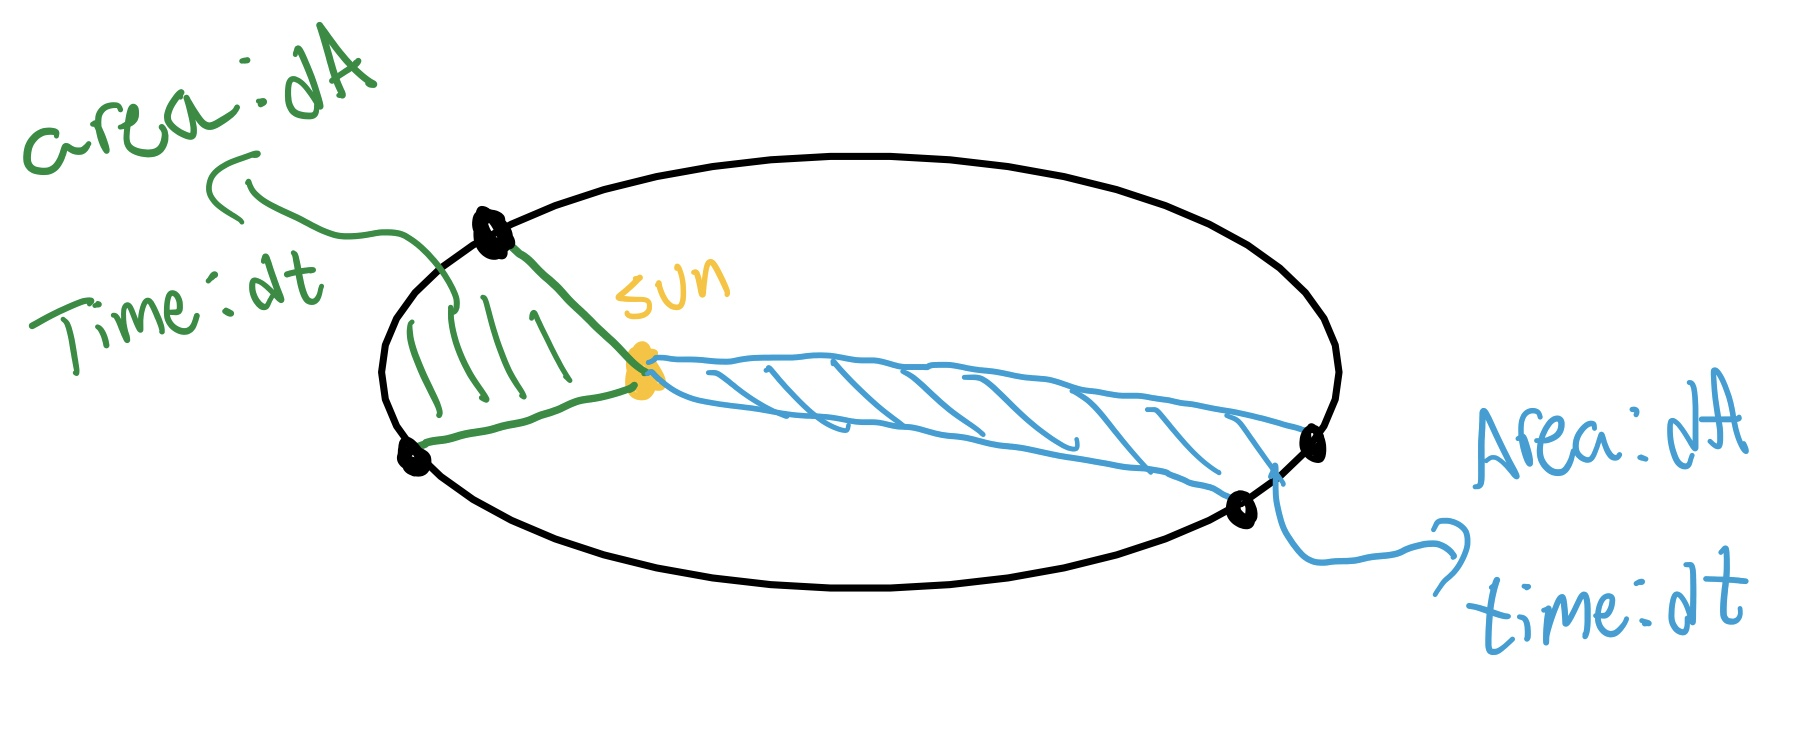
\includegraphics[width=\linewidth]{K2L.jpg}
	\caption{Keeplers second law. Where the area is the same for the same time interval.}
	\label{fig:1bplot}
\end{figure}

The best way to show that the angular momentum is conserved by using Keeplers second law is to make a drawing.


The best way to show that the angular momentum is conserved by using Keeplers second law is to make a drawing:

\begin{figure}[H]
	\centering
	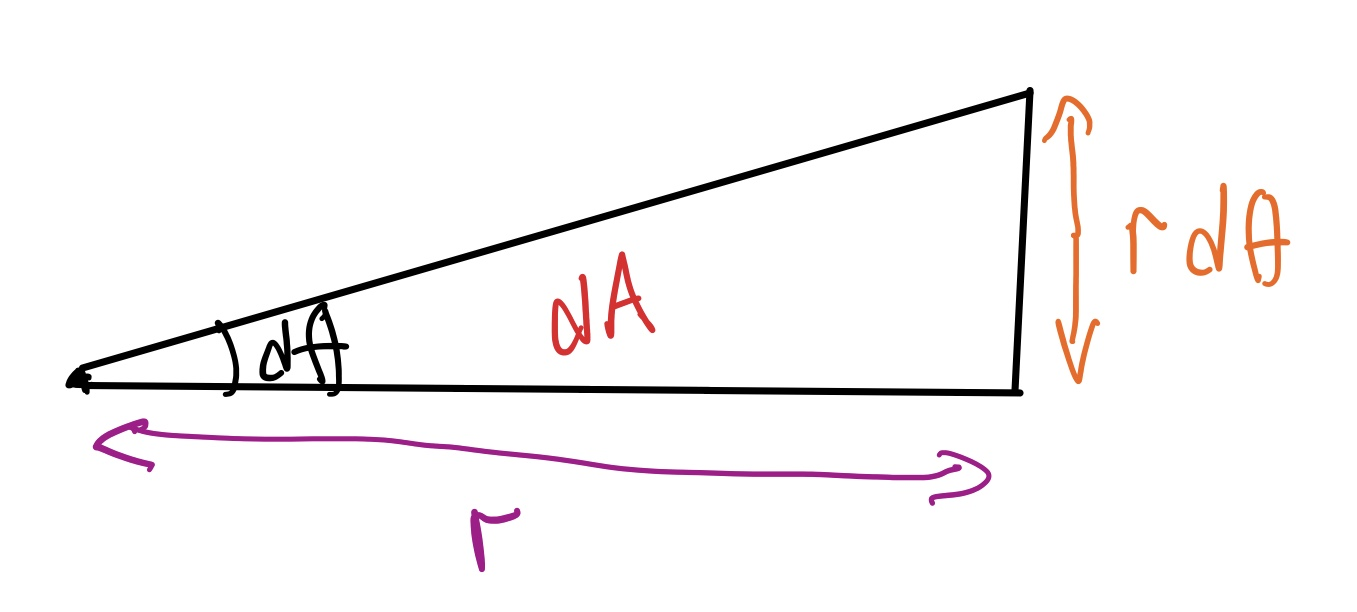
\includegraphics[width=\linewidth]{sketch.jpg}
	\caption{This square is the infinitesimal area dA that the planet has moved by a infinitesimal time interval dt}
	\label{fig:1bplot}
\end{figure}
Figure 2 shows us that the area is 
\begin{align}
    dA=\frac{1}{2}r^2d\theta
\end{align}



\end{multicols}


\clearpage
\appendix % Her kommer appendix.
\section{Calculations} 

\bibliography{References} % Kilder.
\begin{thebibliography}{9}
\bibitem{94}
	Skriv inn kilde her.
\end{thebibliography}
\end{document}
